\documentclass[a4paper]{article}

% Packages
\usepackage{geometry}
\geometry{left=3cm, right=3cm, top=2.54cm, bottom=2.54cm}
\usepackage{graphicx, hyperref, setspace, amsmath, amssymb, titlesec, fancyhdr, multicol, parskip, indentfirst, etoolbox, caption, cite, hyperref, xcolor}

\usepackage{subcaption} % Add to preamble


\usepackage{hyperref}
\hypersetup{
    colorlinks=true,
    linkcolor=blue,
    filecolor=magenta,      
    urlcolor=cyan,
    pdftitle={Overleaf Example},
    pdfpagemode=FullScreen,
    }

\urlstyle{same}

% Title Formatting
\titleformat{\section}{\centering\large\scshape}{\thesection}{1em}{}
\titleformat{\subsection}{\normalsize\bfseries}{\thesubsection.}{1em}{}
\setstretch{1.0} % Keep single spacing
\setlength{\parskip}{6pt} % Space between paragraphs
\titlespacing{\section}{0pt}{6pt}{6pt}
\titlespacing{\subsection}{0pt}{6pt}{6pt}
\titlespacing{\subsubsection}{0pt}{6pt}{6pt}
% Document Title
\title{
    \textbf{YouTube Videos Analysis} 
}

\date{} % No date
\captionsetup{labelfont={small,sc}, textfont={small,sc}}
% Section Numbering
% Define numbering format
\renewcommand{\thesection}{\Roman{section}.}
\renewcommand{\thesubsection}{\textit{\Alph{subsection}.}}
\renewcommand{\thesubsubsection}{\textit{\arabic{subsubsection}.}}
\renewcommand{\thetable}{\Roman{table}} % Set table numbering to Roman
\renewcommand{\thefigure}{\Roman{figure}} % Number figures in Roman numerals

% Make titles italic as well

\titleformat{\subsection}{\normalfont\large\itshape}{\thesubsection}{1em}{}
\titleformat{\subsubsection}{\normalfont\itshape}{\thesubsubsection}{1em}{}


\setcounter{page}{5}

% Fancy Header Configuration
\pagestyle{fancy}
\fancyhf{} % Clear all header/footer fields


% Default Header for Other Pages
\fancyhead[C]{\textbf{Data Science}}

\begin{document}

\maketitle
\vspace{-1.5cm}

% Authors Block
\begin{center}
    \textbf{Mahla Entezari}\\
    \textit{Shahid Beheshti University}\\
    \textit{Tehran, Iran}\\
    \textit{MahlaEntezari.sbu@gmail.com}
    \vfill
\end{center}


% Abstract (single-column)
\begin{abstract}
In the field of data science, each dataset offers the opportunity to uncover meaningful insights. This assignment explores YouTube's video dataset, aiming to extract key trends and patterns related to video engagement, content performance, and audience preferences.
The report chronicles the process of data acquisition, cleaning, and analysis, ultimately revealing insights that can inform content strategies and audience targeting. The goal is to assist stakeholders in making data-driven decisions to optimize video content, increase engagement, and improve overall performance on the platform. 
\end{abstract}


\singlespacing
\setlength{\parskip}{6pt}
\setlength{\parindent}{0.5cm}

 
\begin{multicols}{2}
\setlength{\columnsep}{0.5cm}


\section{Introduction}
YouTube, as one of the largest video-sharing platforms globally, hosts millions of videos and attracts billions of users daily. This project leverages a publicly available YouTube dataset to explore trends and patterns related to video performance, audience engagement, and content categorization. Through the application of exploratory data analysis (EDA) techniques and visualization, the project aims to uncover valuable insights that can enhance content strategies and optimize video performance on the platform.

The primary goal of this project is to: 
\begin{itemize} 
	\item Analyze video engagement metrics, such as views, likes, and comments, across different categories. 
	\item Identify patterns in video performance over time and by category. 
	\item Provide data-driven insights that can inform content creation, audience targeting, and marketing strategies on YouTube. 
\end{itemize}


\section{Dataset} 
\subsection{Trending YouTube Video Statistics} The dataset used for this project, 
\href{https://www.kaggle.com/datasets/datasnaek/youtube-new/}{Trending YouTube Video Statistics}, contains detailed information about YouTube videos, including metrics such as views, likes, comments, and the video’s associated category. The data is designed to help analyze various aspects of video performance, user engagement, and content trends.

Initial data exploration focused on understanding the dataset’s dimensions, identifying missing values, and ensuring data quality before diving into more advanced analysis.

\subsection{YouTube Video Categories and Metadata} In addition to the general video statistics, the dataset also includes metadata related to the categories of the videos, their publish times, and their associated tags. This information allows for deeper insights into how different video categories perform over time, which categories are trending, and how video characteristics such as title length and tags influence viewer engagement.

By analyzing this dataset, we aim to uncover patterns related to video performance, user interactions, and the effectiveness of various content strategies on the platform.






\section{Methods}
 Our methodology began with a thorough data preprocessing phase, followed by a comprehensive exploratory analysis.

\subsection{Data Loading and Exploration} The first step was to load the YouTube dataset and familiarize myself with its structure. The dataset, acquired from a public source on Kaggle, contains detailed video statistics, including views, likes, comments, and category information.\

Using Python's 
\texttt{pandas} library, I quickly inspected the data to understand its dimensions and to identify any immediate issues such as missing values or duplicates.

\subsubsection{Initial Data Inspection} I began by checking the overall shape and data types. This inspection revealed both numerical and categorical variables that required different preprocessing techniques. Missing values and anomalies were identified, setting the stage for a thorough data cleaning process.

\end{multicols} 

\begin{figure}[h]
    \centering
    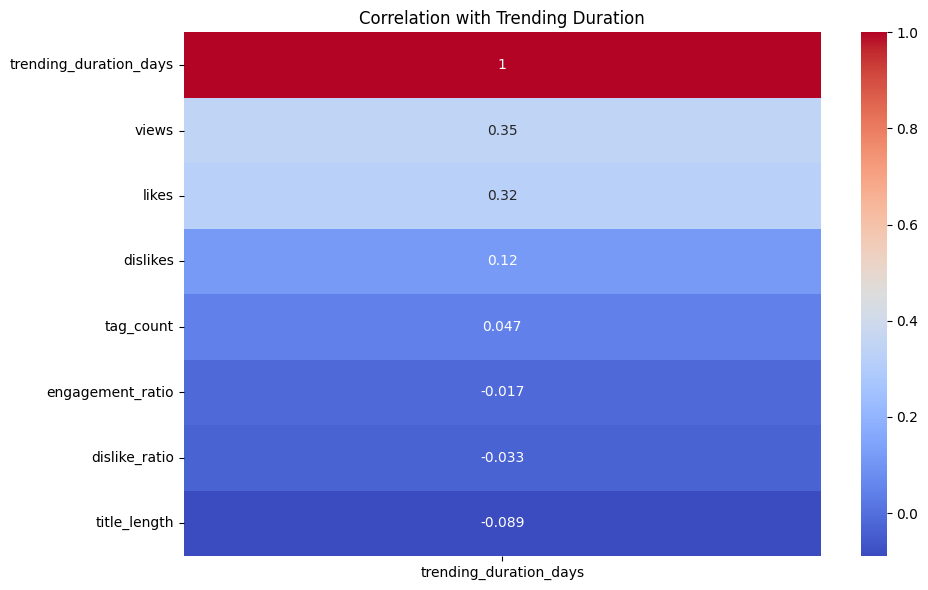
\includegraphics[width=0.7\textwidth]{correlation.png}
    \caption{\textbf{Correlation Matrix}}
    
   The heatmap you've provided shows the correlation between trending duration (in days) \
   
   and various video attributes such as views, likes, title length, etc.

Sustained engagement (views, likes) is a much stronger predictor of longer trending\

 than structural metadata like title length or tag count.

Surprisingly, clickbait phrasing and high engagement ratios \

don’t seem to support longevity they may help a video go viral fast,\

 but not keep it on the trending list.

Dislike ratio has a slight negative impact controversial videos may trend quickly, but drop off faster.

    
    \label{fig:sales}
\end{figure}


\begin{multicols}{2}


\subsubsection{Data Cleaning and Feature Engineering} Real-world datasets often require cleanup. I addressed inconsistencies and missing values by removing duplicates and handling missing entries appropriately. I standardized categorical variables, such as video category names, to ensure uniformity across the dataset.

New features were engineered to enhance the analysis, such as aggregating views by day or week to capture time-based patterns and creating interaction-based variables like the like-to-view ratio. This foundational work was essential for accurate downstream analysis.

\subsection{Uncovering Hidden Patterns} With a cleaned dataset in hand, I proceeded with exploratory data analysis (EDA). The goal was to reveal underlying trends and relationships that could inform content strategies and video performance optimization.

\subsection{Hypothesis Tests} I conducted hypothesis tests to examine the relationship between video features (such as category, title length, and tags) and user engagement (views, likes, comments).


This statistical test evaluates whether there's a significant association between the day a video is published and its likelihood of going viral.
Since the p-value is well below 0.05, we reject the null hypothesis.

Conclusion: There is a statistically significant relationship between the day of the week a video is published and whether it becomes viral.

This finding suggests that publishing day matters—some days are more favorable for videos to gain traction and go viral. Strategic scheduling can be leveraged to maximize visibility and engagement.

\end{multicols}




\section{Visualization}
 Understanding the dataset’s structure and the relationships between variables is crucial in any data analysis. By exploring the data through appropriate visualizations, we can identify trends, detect outliers, and formulate hypotheses that guide further analysis.

To explore relationships between key variables, I employed a variety of visualizations, including scatter plots, bar charts, and heatmaps. These tools helped in uncovering insights into how video performance, such as views, likes, and comments, is influenced by factors like video category, title length, and tags.

For guidance on selecting suitable visualizations, I referred to 
\href{https://www.data-to-viz.com/}{From Data to Viz}, a resource that helps choose the most appropriate chart types based on data characteristics.

By transforming complex numerical relationships into intuitive graphics, each visualization provided a clearer understanding of the data and contributed to uncovering patterns in YouTube video performance.


\begin{figure}[h]
    \centering
    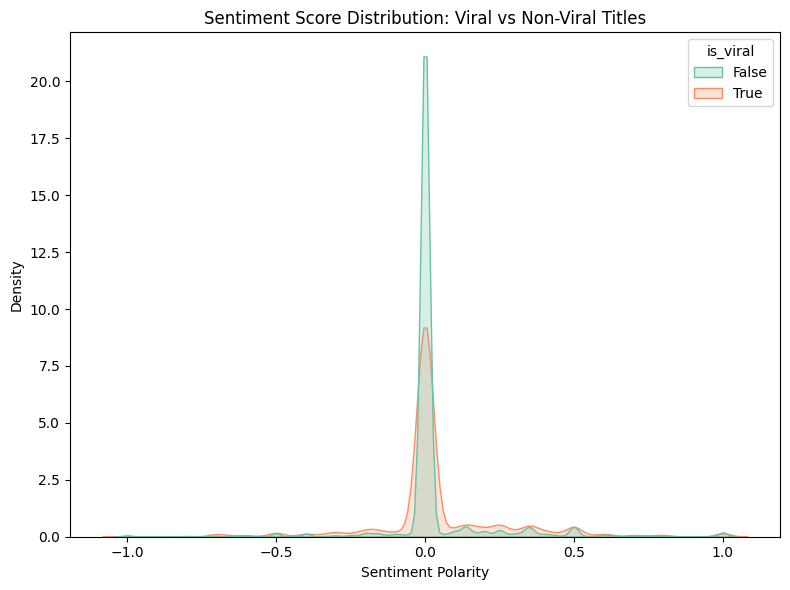
\includegraphics[width=0.5\textwidth]{kde.png}
    \caption{\textbf{KDE plot}}
    This kernel density plot visualizes the distribution of sentiment polarity scores (from -1 to 1) \
    
    for video titles, comparing viral and non-viral YouTube videos.
    
    Sentiment polarity is measured using TextBlob:
    
	-1 = very negative sentiment, 
	0 = neutral, 
	+1 = very positive sentiment, \
	
	The two curves represent the distribution for:
	Viral videos (orange), 
	Non-viral videos (green)
    \label{fig:sales}
\end{figure}

1. Both Groups Are Strongly Centered at Neutral (0).
The vast majority of titles—whether viral or not—have neutral sentiment, likely due to straightforward or descriptive phrasing.

2. Viral Titles Are Slightly More Polarized.
Viral videos show slightly more spread into positive and negative sentiment zones.
This suggests that emotionally charged titles may contribute marginally to virality.

3. Non-Viral Titles Cluster Tightly Around 0.
A narrower, taller peak implies that non-viral titles are more conservative in tone.

While most video titles are neutral, viral titles tend to lean slightly more emotionally charged, possibly to attract attention or provoke curiosity. However, sentiment alone is not a strong predictor of virality—it's one of many contributing factors.

Using emotional language (positive or negative) might slightly boost engagement, but it's not a silver bullet.
Content creators should consider sentiment tone as a stylistic tool, but prioritize relevance and clarity for sustainable success.

\subsection{Histograms}
\begin{figure}[h]
    \centering
    \begin{subfigure}{0.3\textwidth}
        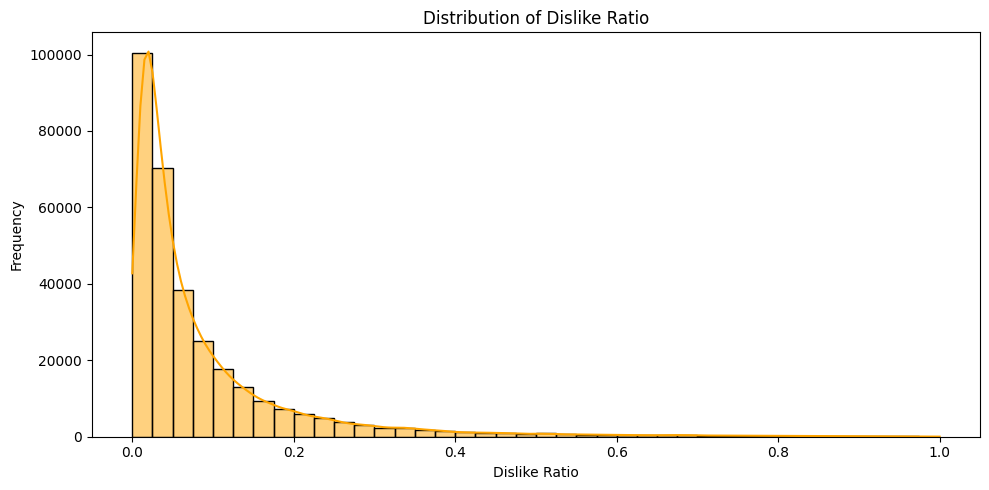
\includegraphics[width=\linewidth]{hist1.png}
        \caption{Distribution of Dislike Ratio}
        \label{fig:sub1}
    \end{subfigure}
    \hfill
    \begin{subfigure}{0.3\textwidth}
        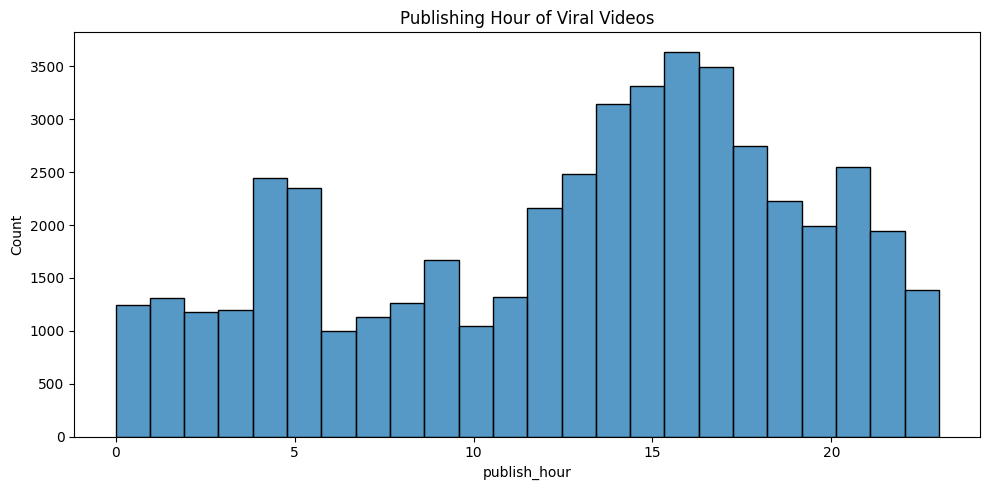
\includegraphics[width=\linewidth]{hist2.png}
        \caption{Publishing Hour of Viral Videos}
        \label{fig:sub2}
    \end{subfigure}
    \hfill
    \begin{subfigure}{0.3\textwidth}
        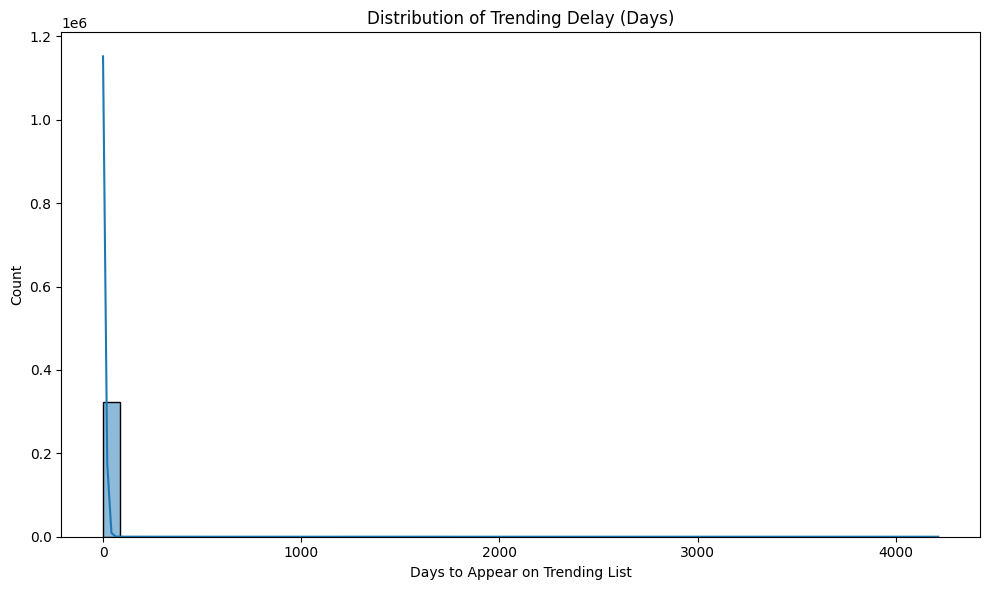
\includegraphics[width=\linewidth]{hist3.png}
        \caption{IDistribution of Trending Delay}
        \label{fig:sub3}
    \end{subfigure}
    \caption{Some histograms for visualization}
    \label{fig:multi}
\end{figure}


\begin{multicols}{2} 

First histogram illustrates the distribution of dislike ratios for trending YouTube videos.

1. Majority of Videos Have Low Dislike Ratios
Most trending videos have a dislike ratio below 0.1, meaning over 90 of user engagement is positive (likes).
Indicates that content which trends is generally well-received or positively curated by YouTube’s algorithms.

2. Right-Skewed Distribution
The plot shows a right-skewed (positively skewed) distribution:
A long tail of videos with higher dislike ratios (0.2 and above), but infrequent.

A small number of videos receive 20–40 dislikes, possibly due to:
Controversial topics
Misleading thumbnails or titles (clickbait)
Poor quality or spam content

3. Outliers Beyond 0.5
Very few videos exceed a dislike ratio of 0.5, meaning they were disliked more than liked.
These are rare but could signal controversy, public backlash, or poor relevance.

Use dislike ratio as a feature to identify:
Controversial videos (potential virality or reputation risk)
Misleading content (possible flag for moderation or review)



The second histogram displays the distribution of publishing hours for videos that achieved viral status (defined as views more than 1,000,000).

1. Peak Viral Publishing Times:
Viral videos are most frequently published during:
Afternoon hours (12:00 PM – 18:00 PM), peaking around 16:00.
A secondary cluster appears around 4:00–5:00 AM, possibly due to scheduled global releases or optimization for early risers in specific regions.

2. Early Morning Hours Have Fewer Viral Videos
Very few viral videos are published between 1:00 AM – 6:00 AM, suggesting that this timeframe might be less favorable for virality—unless targeting international audiences.

While engaging content is key, timing matters too—especially for maximizing visibility in YouTube’s recommendation system. Afternoon publishing aligns with:
User availability after school/work
YouTube's algorithm surfacing fresh uploads



And the last one shows that most videos appear on the trending list within 0 to 10 days after upload, with a very sharp peak at Day 0 (same-day trending).

The distribution has a long right tail, suggesting a small number of videos take much longer to trend (weeks or even years).
Some extreme delays (e.g., nore than 1000 days) may be anomalies or archival uploads that resurfaced.



\end{multicols}

\subsection{Bar Plots}
\begin{figure}[h]
    \centering
    \begin{subfigure}{0.32\textwidth}
        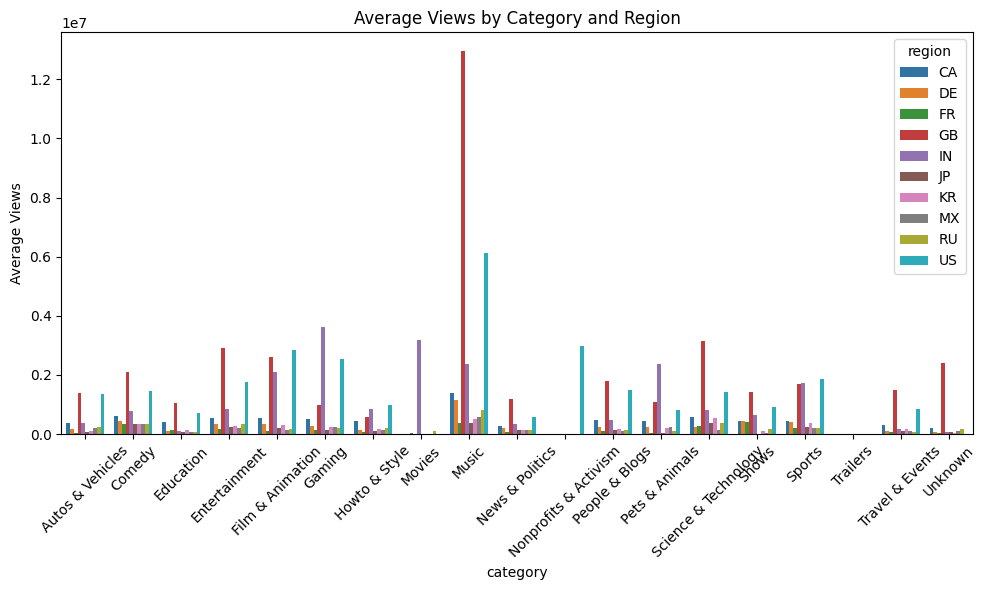
\includegraphics[width=\linewidth]{bar1.png}
        \caption{Average Views by Category and Region}
        \label{fig:sub1}
    \end{subfigure}
    \hfill
    \begin{subfigure}{0.32\textwidth}
        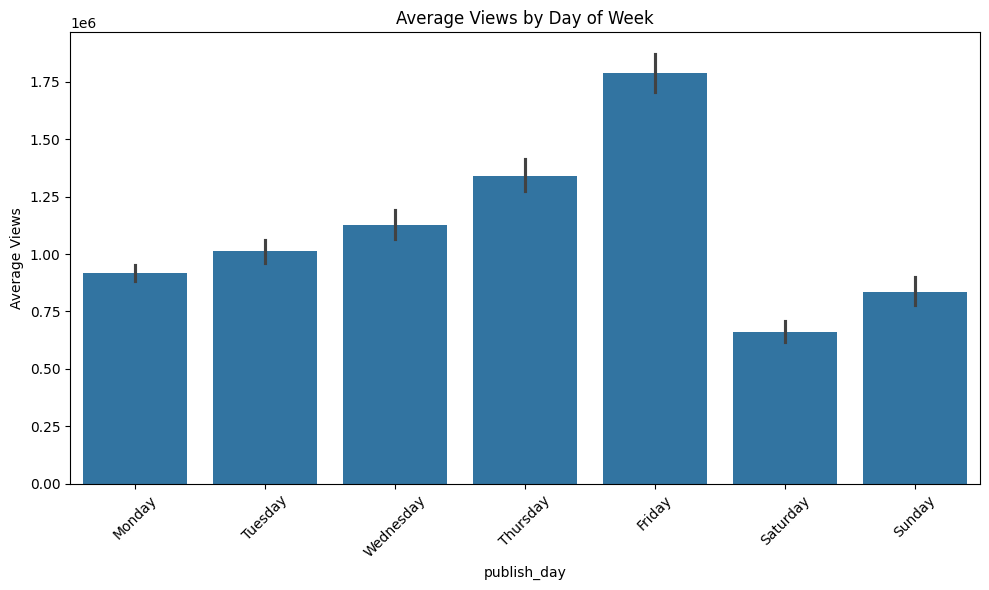
\includegraphics[width=\linewidth]{bar3.png}
        \caption{Average Views by Day of Week}
        \label{fig:sub2}
    \end{subfigure}
    \hfill
    \begin{subfigure}{0.32\textwidth}
        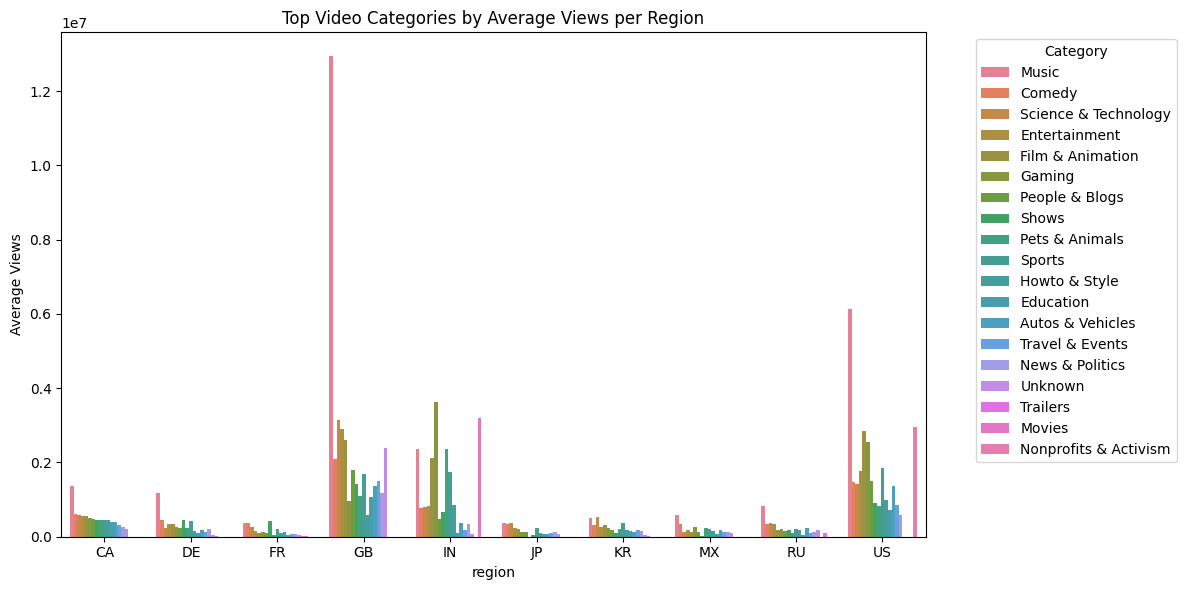
\includegraphics[width=\linewidth]{bar2.png}
        \caption{Top Video Categories by Average View per Region}
        \label{fig:sub3}
    \end{subfigure}
    \hfill
    \begin{subfigure}{0.32\textwidth}
        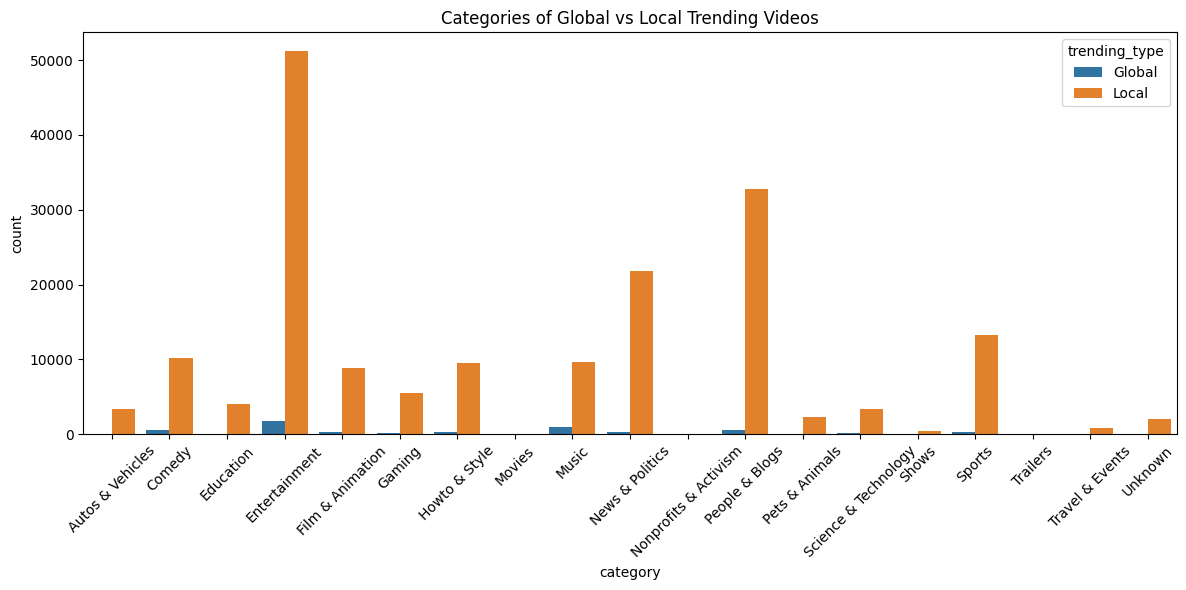
\includegraphics[width=\linewidth]{bar4.png}
        \caption{Categries of Global vs Local Trending Videos}
        \label{fig:sub4}
    \end{subfigure}
    \caption{Some bar plots for visualization}
    \label{fig:multi}
\end{figure}



\begin{multicols}{2} 


The first grouped bar chart compares the average view count across different content categories and regions (e.g., US, GB, IN, etc.).

1. Music Dominates
The Music category stands out massively across multiple regions.
In particular, Great Britain (GB) and the United States (US) show extreme spikes in average views — GB exceeding 12 million views, and US over 6 million.
This suggests music videos have strong global appeal and high replayability.

2. Regional Preferences Are Clear
India (IN) shows high engagement across Gaming, Entertainment, and Howto \& Style.
Korea (KR) shows peaks in Gaming, Film \& Animation, and Music.
Russia (RU) and France (FR) have generally lower average views across categories, possibly indicating more fragmented content consumption or fewer trending uploads.

3. Entertainment \& Film
Categories like Entertainment, Film \& Animation, and Gaming also show relatively high averages in several regions — particularly IN, KR, and US.

4. Low Engagement Categories
Categories such as Nonprofits \& Activism, Pets \& Animals, and Science \& Technology show consistently lower average views across most regions, suggesting niche audiences or lower trending potential.

5. Cultural Variability
The diversity of spikes indicates regional cultural preferences. For instance:

- News \& Politics is more viewed in US and KR\
- People \& Blogs peaks more in IN\
- Education has modest popularity across all regions but never spikes\
- To maximize reach globally, focus on Music, Gaming, and Entertainment.

If targeting specific regions:\
- GB/US: Prioritize Music and News\
- IN: Consider Gaming, People \& Blogs, and Film\
- KR: Lean into Film \& Animation, Music, and Gaming





The second bar chart visualizes the average number of views that trending YouTube videos receive based on the day of the week they are published.

1. Friday is the Peak Engagement Day
Videos published on Friday receive the highest average views by far — over 1.75 million on average.

This may be due to:
- Increased user activity as the weekend begins
- More leisure time to explore and share content
- Platforms potentially boosting end-of-week uploads

 2. Gradual Build-Up During the Week
Views increase steadily from Monday to Thursday, suggesting:
Mid-week is a good window for building momentum
Audiences are active and engaged leading up to the weekend

3. Weekends Underperform
Saturday and Sunday show a noticeable drop, especially Saturday (lowest).

Possible reasons:
- Competing real-world activities reduce screen time
- Algorithms may favor weekday uploads for initial traction

 4. Statistical Implications
Although this chart shows a clear trend by weekday, the Chi-Square test earlier showed no statistically significant association.
That suggests other variables (e.g., content type, country, promotion) may play a larger role in virality.







The third grouped bar chart provides a regional breakdown of average video views by content category, showing how content popularity varies across countries like the US, GB, IN, JP, and more.


1. Music Dominates Across Regions
Music consistently earns the highest average views across nearly all regions, with Great Britain (GB) showing a massive spike (over 12 million average views).
US, IN, and KR also show significant popularity for music content.
This highlights music’s universal appeal and strong shareability across cultures.

2. Nonprofits \& Activism is a Standout in GB and US
GB and US both show high engagement in the Nonprofits \& Activism category, possibly influenced by:\
- Political campaigns
- Charity drives
- Social justice initiatives

3. India’s Unique Profile
Gaming is exceptionally popular in India, even rivaling entertainment content.
Movies and Film \& Animation also attract substantial views.
Suggests that India’s trending videos are skewed toward visual, cinematic, and interactive formats.

4. Diverse Tastes in US, Korea, and GB
US shows strong viewership in:\
- Music
- News \& Politics
- Movies
- Korea has high averages across:
- Music
- Entertainment
- Film \& Animation

5. Lower View Averages in Regions like JP, FR, RU
Categories in Japan, France, and Russia tend to have lower average views, indicating either:
A more evenly distributed trending pattern (less viral spikes)

Regional content preferences that don’t rely on large-scale virality.






The last bar chart compares the number of videos trending globally (in more than one country) versus locally (in a single country) across different content categories.

Entertainment, Music, and News \& Politics dominate both globally and locally, but:
- Entertainment clearly drives the largest volume of local virality.
- Music and News \& Politics show more global reach, making them leading candidates for cross-border engagement.
- People \& Blogs, Comedy, and How-to content trend primarily locally, suggesting cultural or language-specific appeal.

Videos in certain categories have higher chances of "spilling over" into multiple countries—especially those with universal appeal like music or global news.
Categories with local flavor (like People \& Blogs) tend to go viral within regions rather than internationally.

If the goal is international virality, producing content in globally engaging formats (music, breaking news, etc.) may be more effective than locally focused or culturally niche content.\





\end{multicols}



\subsection{Scatter Plots}
\begin{figure}[h]
    \centering
        \begin{subfigure}{0.3\textwidth}
        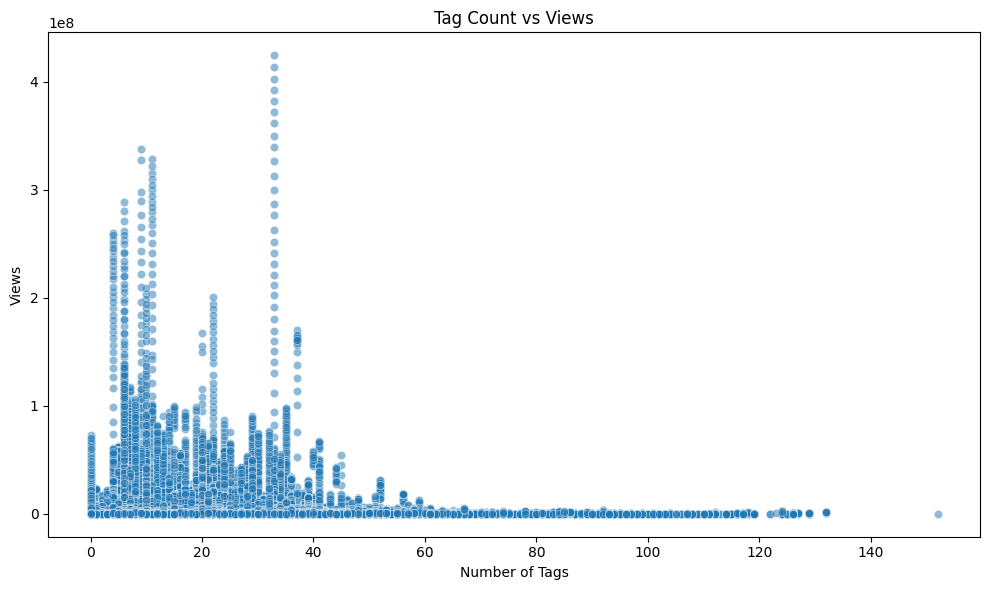
\includegraphics[width=\linewidth]{other4.png}
        \caption{Tag Count vs Views}
        \label{fig:sub4}
    \end{subfigure}
    \hfill
    \begin{subfigure}{0.3\textwidth}
        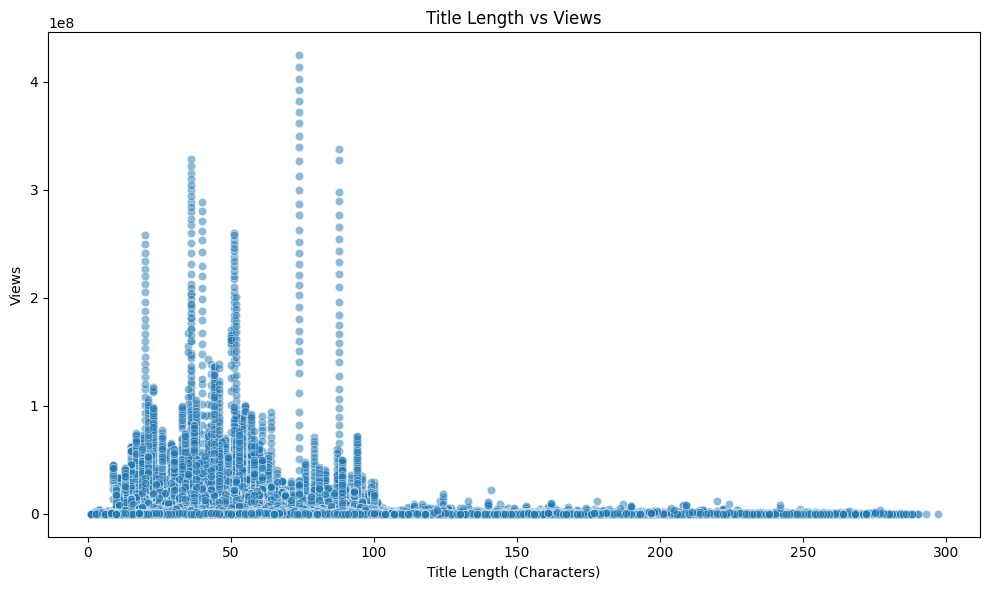
\includegraphics[width=\linewidth]{other5.png}
        \caption{Title Length vs Views}
        \label{fig:sub5}
    \end{subfigure}
    \hfill
    \begin{subfigure}{0.3\textwidth}
        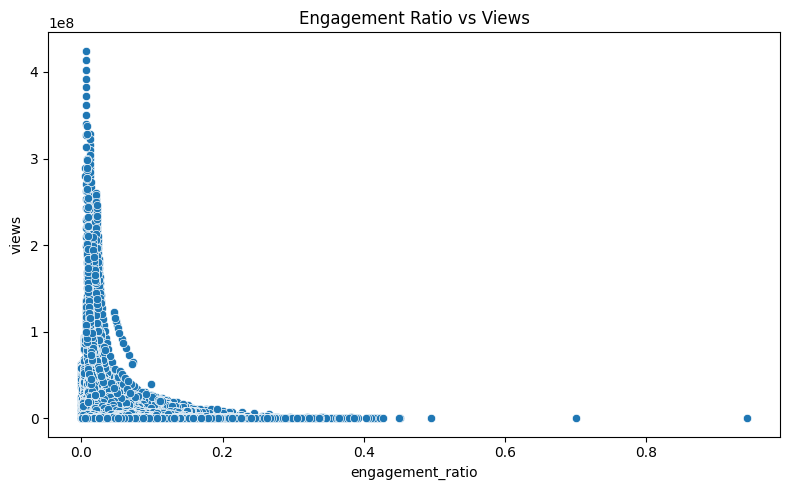
\includegraphics[width=\linewidth]{other7.png}
        \caption{Engagement Ratio vs Views}
        \label{fig:sub5}
    \end{subfigure}
    \hfill
    \begin{subfigure}{0.3\textwidth}
        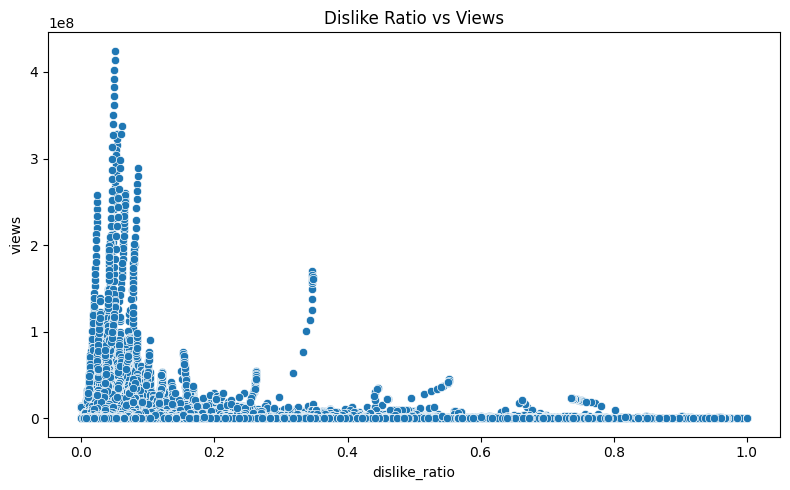
\includegraphics[width=\linewidth]{other8.png}
        \caption{Dislike Ratio vs Views}
        \label{fig:sub5}
    \end{subfigure}
    \label{fig:multi}
\end{figure}

\begin{multicols}{2} 

The first scatter plot explores the relationship between the number of tags used in a video (tagcount) and its view count, across all trending YouTube videos in the dataset.
1. Most Popular Videos Use ~10–30 Tags
A dense cluster of high-performing videos sits in the 10–30 tag range.
These videos have view counts ranging from a few thousand to hundreds of millions.
This suggests a possible sweet spot for metadata optimization.

2. No Clear Linear Correlation
There’s no strong linear relationship between tag count and views — more tags don’t guarantee more views.
However, too few or too many tags (e.g., 0–5 or over 60) are rarely associated with very high view counts.

3. Diminishing Returns After 40+ Tags
After around 40 tags, videos are almost never highly viewed.
This may be due to:\
- Tag stuffing, which could reduce content quality signals
- Algorithmic penalties or irrelevance

4. Some Anomalies
A small number of outliers with extremely high views appear even at 35+ tags — possibly music videos or promotional content from top creators.



The second plot investigates the relationship between a video’s title length (in characters) and its view count across all trending YouTube videos.

1. Sweet Spot: 30–70 Characters
Most high-performing videos (those with tens to hundreds of millions of views) have titles between 30 and 70 characters.
This range is long enough to be descriptive, yet concise enough to remain readable and clickable.

2. No Linear Relationship
There is no strong correlation between title length and view count.
Both short and long titles can trend — but the majority of highly viewed videos are clustered in a mid-length range.

3. Very Long Titles (>100 Characters) Underperform
Titles longer than 100 characters show significantly fewer high-view videos.
These may be:\
-Truncated in search or feed previews
- Perceived as spammy or overwhelming

4. Outliers at 60–90 Characters
Some of the most viral videos (over 100M+ views) use titles in this range.
Suggests well-optimized titles may pack keywords and intrigue into a medium-length frame.



The third one visualizes the relationship between a video’s engagement ratio (likes per views) and its total view count.

1. Inverse Relationship
The plot clearly shows a strong inverse pattern:
- As views increase, the engagement ratio (likes per view) tends to decrease.
- Highly viewed videos have much lower engagement ratios, often below 1\%.

 2. High Engagement not equal to High Reach
Some videos with very high engagement ratios (>10\%) exist — but they rarely go viral.

This suggests:\
- These may be niche, targeted content with strong appeal to small audiences.
- Viral videos attract a broader audience with lower relative engagement.

 3. Scalable Content = Wide but Shallow
Viral success appears to trade off depth of interaction (engagement) for breadth of exposure (views).

Algorithms may favor content that draws broad appeal, even if fewer people interact deeply.
Engagement ratios are valuable for measuring community connection or audience enthusiasm, but they shouldn’t be the sole metric for evaluating content success on platforms like YouTube. Viral visibility often depends more on clicks, watch time, and shareability than raw likes.



The last scatter plot illustrates the relationship between a video’s dislike ratio (dislikes / (likes + dislikes)) and its total view count.

1. Dislike Ratio Increases, Views Decrease
A clear negative correlation exists between dislike ratio and views:
Most high-view videos have low dislike ratios, generally below 0.2 (20\%).
As dislike ratio approaches 0.5 or higher, views tend to fall sharply.

2. Controversy Doesn’t Scale Well
Even though some controversial videos (with dislike ratio > 0.3) reach millions of views, they are:
- Far fewer in number
- Highly variable in view performance
This confirms that controversial or polarizing content may attract attention, but rarely achieves consistent virality.

3. Very High Dislike Ratios Are Outliers
Content with dislike ratios nearing 1.0 (i.e., almost all reactions are dislikes) is extremely rare and generally performs poorly in terms of viewership.
These may represent scams, misleading content, or algorithmically penalized uploads.
To maximize visibility and reach, content creators should strive to maintain a low dislike ratio, suggesting they are:\
- Delivering on expectations
- Avoiding misleading or polarizing elements
- Creating positive viewer experiences



\end{multicols}

\subsection{Other Plots}
\begin{figure}[h]
    \centering
    \begin{subfigure}{0.3\textwidth}
        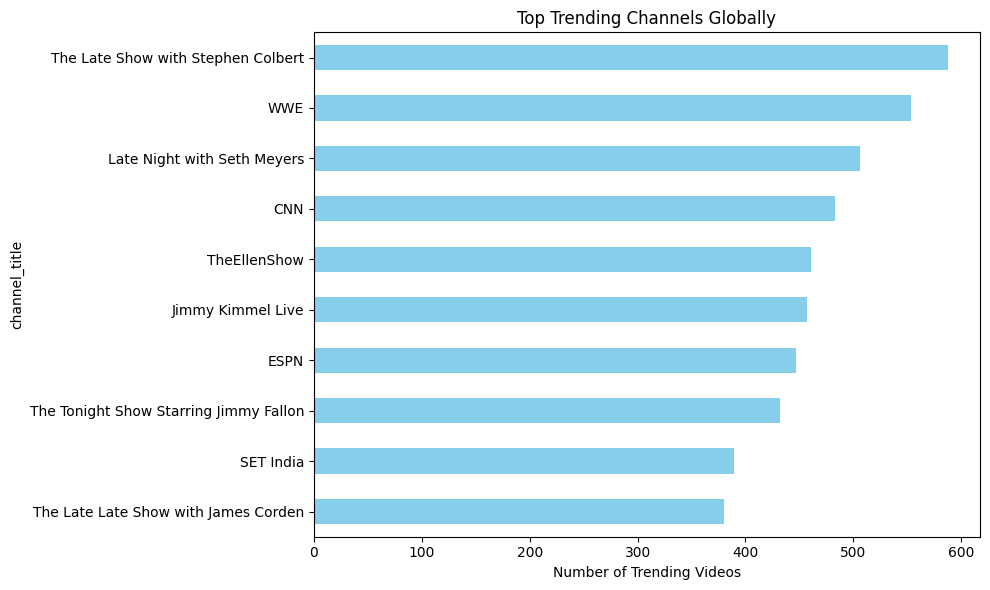
\includegraphics[width=\linewidth]{other1.png}
        \caption{Top Trending Channels Globally}
        \label{fig:sub1}
    \end{subfigure}
    \hfill
    \begin{subfigure}{0.3\textwidth}
        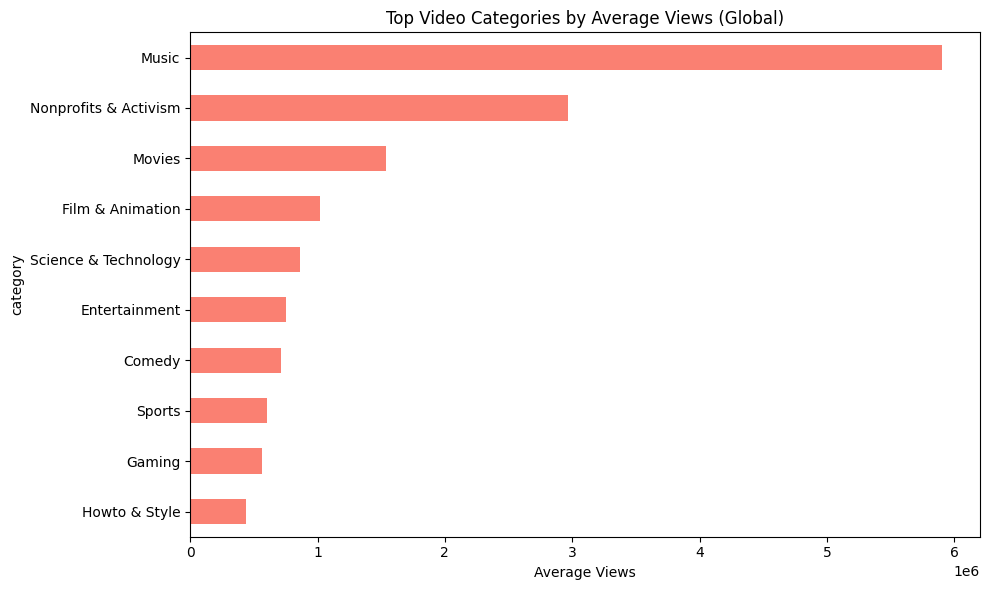
\includegraphics[width=\linewidth]{other2.png}
        \caption{Top Video Categories by Average Views (Global)}
        \label{fig:sub2}
    \end{subfigure}
    \hfill
    \begin{subfigure}{0.3\textwidth}
        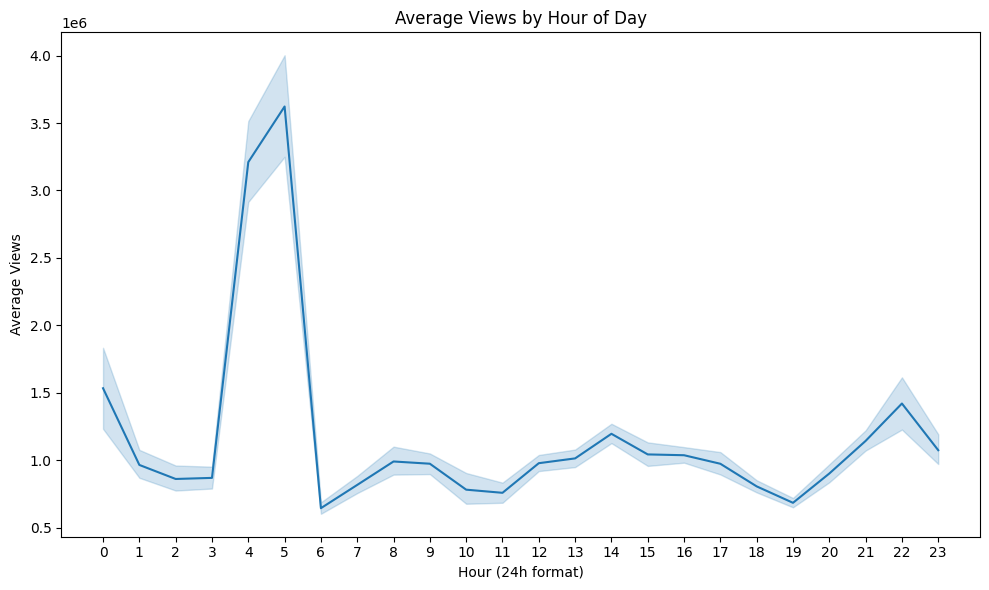
\includegraphics[width=\linewidth]{other3.png}
        \caption{Average View by Hour of Day}
        \label{fig:sub3}
    \end{subfigure}
    \hfill
    \begin{subfigure}{0.3\textwidth}
        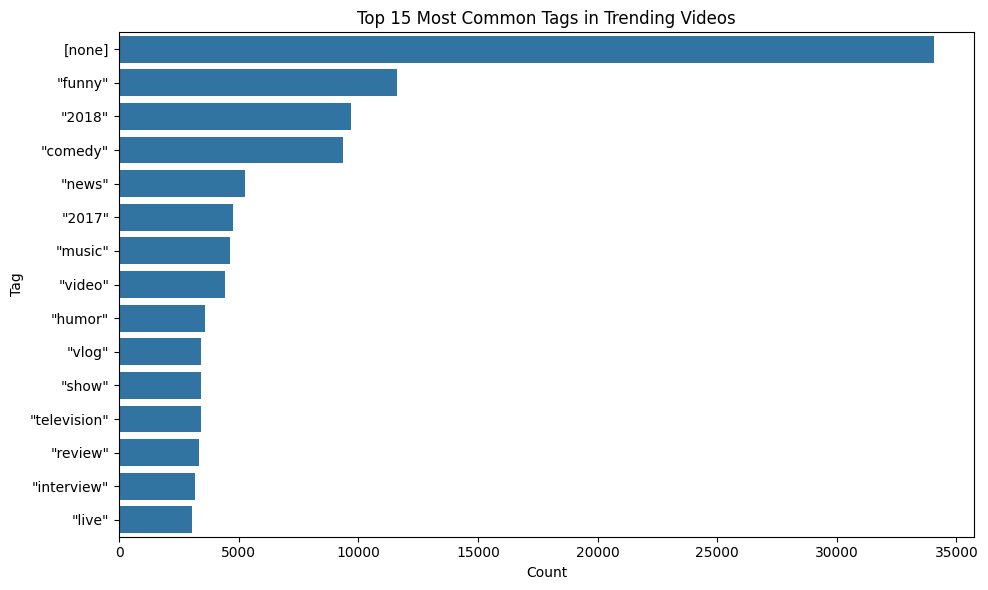
\includegraphics[width=\linewidth]{other6.png}
        \caption{Top 15 Most Common Tags in Trending Videos}
        \label{fig:sub6}
    \end{subfigure}
    \hfill
    \begin{subfigure}{0.3\textwidth}
        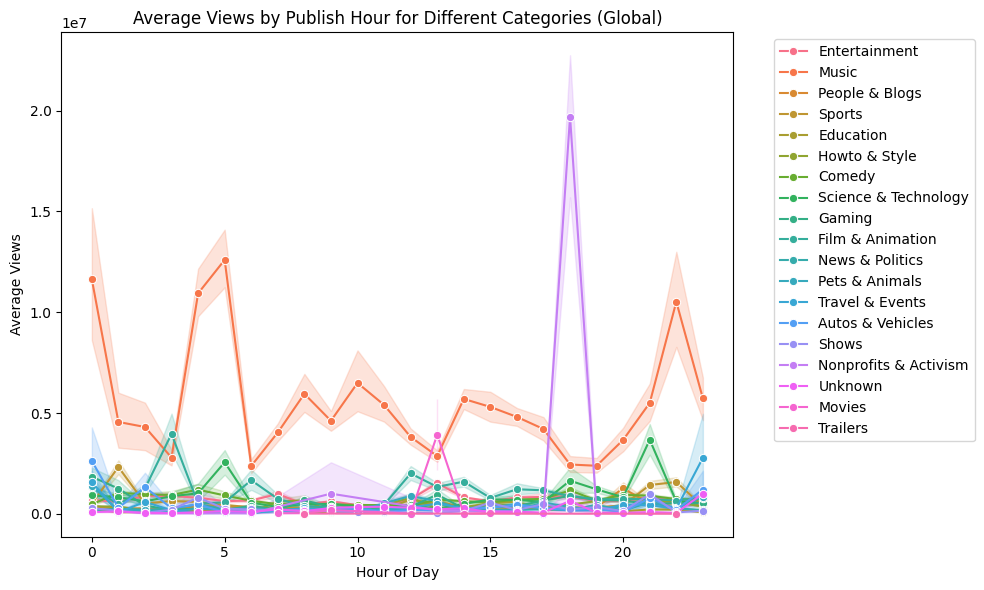
\includegraphics[width=\linewidth]{other9.png}
        \caption{Average Views by Publish Hour for Different Categories}
        \label{fig:sub5}
    \end{subfigure}
    \hfill
    \begin{subfigure}{0.3\textwidth}
        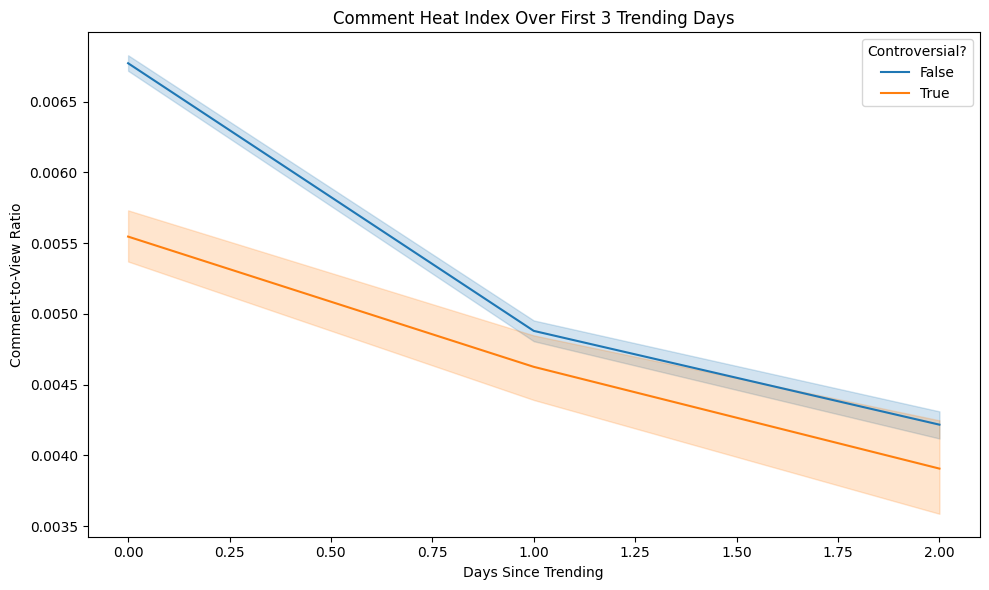
\includegraphics[width=\linewidth]{other10.png}
        \caption{Comment Heat Idex Over First 3 Trending Days}
        \label{fig:sub5}
    \end{subfigure}
    \begin{subfigure}{0.3\textwidth}
        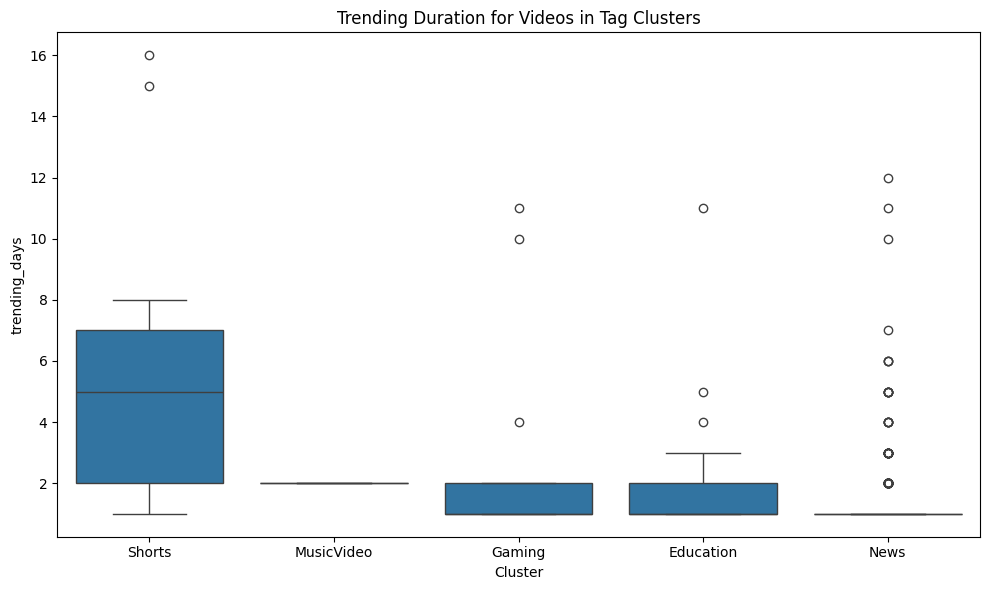
\includegraphics[width=\linewidth]{other11.png}
        \caption{Trending Duration for Videos in Tag Clusters}
        \label{fig:sub5}
    \end{subfigure}
    \hfill
    \caption{Some box plots for visualization}
    \label{fig:multi}
\end{figure}


\begin{multicols}{2} 


\section{Results}

This analysis aimed to uncover key trends and insights from a dataset of trending YouTube videos, focusing on engagement metrics, content performance, and user preferences. The key findings from the data analysis are as follows:

\subsection{Video Engagement and Categories}
The analysis of video engagement metrics, such as views, likes, comments, and dislike ratios, revealed a strong correlation between sustained engagement (views and likes) and longer periods of trending. Videos that maintain high engagement tend to stay on the trending list for longer durations. Interestingly, structural metadata like title length and tag count did not significantly impact the video’s ability to stay trending. This suggests that content quality and audience engagement are more critical factors than technical elements in a video’s success on YouTube.

\subsection{Influence of Sentiment and Emotion in Titles}
A Kernel Density Estimate (KDE) plot comparing viral and non-viral video titles based on sentiment polarity showed that both viral and non-viral video titles were predominantly neutral in sentiment. However, viral titles had a slightly higher spread into both positive and negative sentiment, suggesting that emotionally charged or attention-grabbing titles might contribute to a video’s virality. While sentiment was not a strong predictor of virality, it was clear that emotional language could marginally boost engagement.

\subsection{Dislike Ratios and Content Controversy}
The distribution of dislike ratios indicated that most trending videos had a low dislike ratio, with the majority of engagement being positive. However, there were a small number of videos that exhibited higher dislike ratios, particularly those associated with controversial or clickbait content. These videos tend to trend quickly but lose traction faster, suggesting that while controversial content may attract initial attention, it is less sustainable in the long term.

\subsection{Publishing Time and Video Virality}
The analysis of publishing time revealed that videos published in the afternoon (12:00 PM – 6:00 PM) were more likely to achieve viral status, with a secondary peak around early morning hours (4:00–5:00 AM), possibly due to global releases. Videos published during the night (1:00 AM – 6:00 AM) were less likely to go viral. This finding highlights the importance of timing in maximizing visibility, particularly for content creators aiming to gain traction quickly on YouTube.

\subsection{Regional Trends and Content Preferences}
The analysis of video views by region revealed strong regional preferences. Music videos were particularly popular in regions like the US and Great Britain, with average views exceeding 12 million in Great Britain alone. Other categories such as Gaming, Entertainment, and Howto \& Style were highly engaging in regions like India and Korea. These regional preferences suggest that content creators should tailor their strategies to regional tastes to enhance engagement. For instance, music and entertainment content should target global audiences, while Gaming and Film \& Animation might perform better in specific regions like India and Korea.

\subsection{Effect of Video Tags on Views}
The relationship between the number of tags used in a video and its view count showed that the most successful videos typically used between 10 and 30 tags. While the correlation was not linear, using too few or too many tags (e.g., fewer than five or more than 40) did not seem to lead to higher view counts. This suggests that there is an optimal range for tag usage, beyond which diminishing returns set in. This finding is useful for video creators to optimize metadata without overloading their content with irrelevant tags.

\subsection{Influence of Title Length on Views}
The scatter plot analysis of title length versus views revealed that videos with titles ranging from 30 to 70 characters received the highest average views. Titles shorter than 30 characters or longer than 100 characters tended to perform less well. This suggests that video titles should strike a balance between being informative yet concise to capture the attention of potential viewers.

\subsection{Global vs. Local Trends}
A comparison of global versus local trending videos highlighted that categories like Music, Entertainment, and News \& Politics had a broader international appeal. In contrast, categories like People \& Blogs and Comedy tended to trend more locally, suggesting that some content categories are more suited for regional audiences. This information could guide content creators in targeting either local or global audiences based on the nature of their content.

\subsection{Conclusion}
This project provided valuable insights into YouTube video performance, emphasizing the importance of engagement metrics, timing, and sentiment in video success. Content creators can use these findings to optimize their video strategies, from choosing the right publishing time to crafting attention-grabbing titles and utilizing an optimal number of tags. Moreover, the analysis revealed the significant impact of regional preferences on content virality, offering guidance on how to tailor content for specific audiences. By leveraging these data-driven insights, content creators can maximize their chances of success on the platform and engage a wider audience.




\begin{thebibliography}{9}

\bibitem{dataset}
Dataset available on Kaggle: ``YouTube Dataset'' by MahlaEn. \textit{Available at:} \url{https://www.kaggle.com/datasets/datasnaek/youtube-new/}.

\bibitem{dataset}
Plots for data visualization. \textit{Available at:} \url{https://www.data-to-viz.com/}.


\bibitem{Statistics}
cole nussbaumer knaflic. \textit{Storytelling with data } a data visualization guide for business.

\end{thebibliography}

\end{multicols}
\end{document}